\subsection{Strecken, Verschieben und Spiegeln von Graphen}

\subsubsection{Strecken und Stauchen}

\underline{Vertikale Streckung:} \\
$f(x) \rightarrow\ a\cdot f(x)$ \\
$a > 1$ ist eine \textbf{Streckung} \\
$a < 1$ ist eine \textbf{Stauchung} 

\parbox[t]{0.32\textwidth}{
    \scalebox{0.6}{
        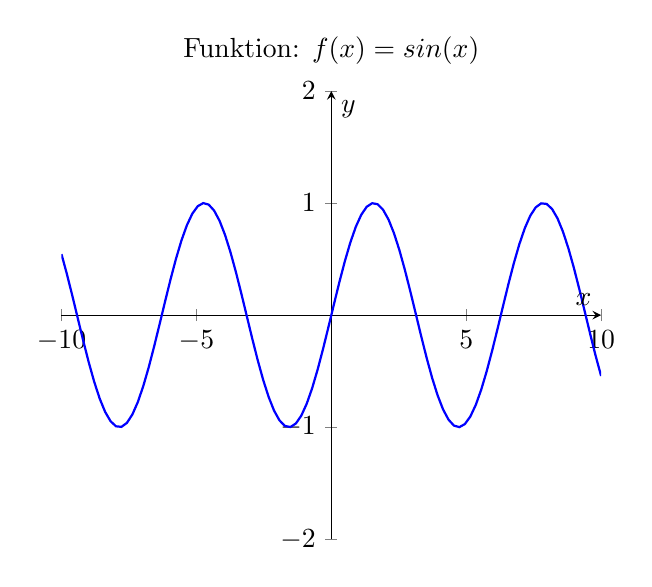
\begin{tikzpicture}
            \begin{axis}[
                axis lines=middle,
                xlabel={$x$},
                ylabel={$y$},
                title={Funktion: $f(x) = sin(x)$},
                %grid=major,
                domain=-10:10, % Range for x
                samples=100, % Number of samples for smoothness
                xmin=-10,xmax=10,ymin=-2,ymax=2
                ]
                \addplot[blue, thick] {sin(deg(x))};
            \end{axis}
        \end{tikzpicture}
    }
}
\hfill
\parbox[t]{0.32\textwidth}{
    \scalebox{0.6}{
        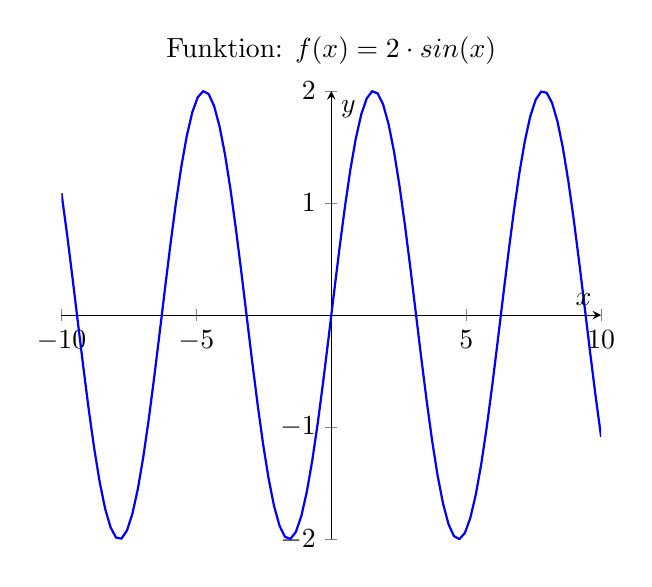
\begin{tikzpicture}
            \begin{axis}[
                axis lines=middle,
                xlabel={$x$},
                ylabel={$y$},
                title={Funktion: $f(x) = 2\cdot sin(x)$},
                %grid=major,
                domain=-10:10, % Range for x
                samples=100, % Number of samples for smoothness
                xmin=-10,xmax=10,ymin=-2,ymax=2
                ]
                \addplot[blue, thick] {2*sin(deg(x))};
            \end{axis}
        \end{tikzpicture}
    }
}
\hfill
\parbox[t]{0.32\textwidth}{
    \scalebox{0.6}{
        \begin{tikzpicture}
            \begin{axis}[
                axis lines=middle,
                xlabel={$x$},
                ylabel={$y$},
                title={Funktion: $f(x) = 0.2 \cdot sin(x)$},
                %grid=major,
                domain=-10:10, % Range for x
                samples=100, % Number of samples for smoothness
                xmin=-10,xmax=10,ymin=-2,ymax=2
                ]
                \addplot[blue, thick] {0.2*sin(deg(x))};
                %\legend{$y = e^x$}
            \end{axis}
        \end{tikzpicture}
    }
}

\underline{Horzontale Streckung:} \\
$f(x) \rightarrow\ f(x \cdot b)$ \\
$b > 1$ ist eine \textbf{Stauchung} \\
$0 < b < 1$ ist eine \textbf{Streckung} 

\parbox[t]{0.32\textwidth}{
    \scalebox{0.6}{
        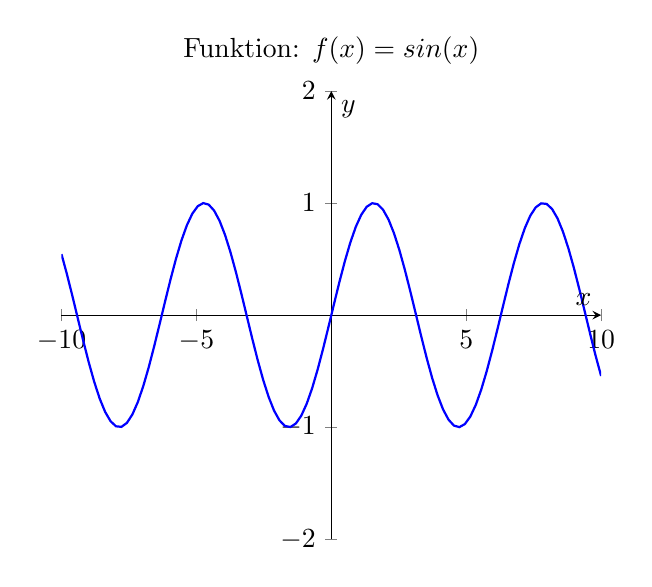
\begin{tikzpicture}
            \begin{axis}[
                axis lines=middle,
                xlabel={$x$},
                ylabel={$y$},
                title={Funktion: $f(x) = sin(x)$},
                %grid=major,
                domain=-10:10, % Range for x
                samples=100, % Number of samples for smoothness
                xmin=-10,xmax=10,ymin=-2,ymax=2
                ]
                \addplot[blue, thick] {sin(deg(x))};
            \end{axis}
        \end{tikzpicture}
    }
}
\hfill
\parbox[t]{0.32\textwidth}{
    \scalebox{0.6}{
        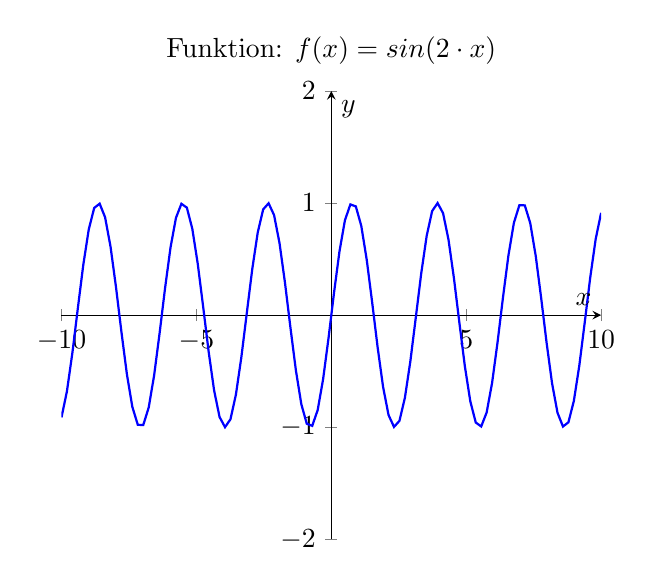
\begin{tikzpicture}
            \begin{axis}[
                axis lines=middle,
                xlabel={$x$},
                ylabel={$y$},
                title={Funktion: $f(x) = sin(2\cdot x)$},
                %grid=major,
                domain=-10:10, % Range for x
                samples=100, % Number of samples for smoothness
                xmin=-10,xmax=10,ymin=-2,ymax=2
                ]
                \addplot[blue, thick] {sin(deg(2*x))};
                %\legend{$y = e^x$}
            \end{axis}
        \end{tikzpicture}
    }
}
\hfill
\parbox[t]{0.32\textwidth}{
    \scalebox{0.6}{
        \begin{tikzpicture}
            \begin{axis}[
                axis lines=middle,
                xlabel={$x$},
                ylabel={$y$},
                title={Funktion: $f(x) = sin(0.3\cdot x)$},
                %grid=major,
                domain=-10:10, % Range for x
                samples=100, % Number of samples for smoothness
                xmin=-10,xmax=10,ymin=-2,ymax=2
                ]
                \addplot[blue, thick] {sin(deg(0.3*x))};
            \end{axis}
        \end{tikzpicture}
    }
}

\subsubsection{Verschieben}
\underline{Vertikale Verschiebung:} \\
$f(x) \rightarrow\ f(x) + c$ \\
$c > 0$ eine Verschiebung nach oben \\
$c < 0$ eine Verschiebung nach unten

\parbox[t]{0.32\textwidth}{
    \scalebox{0.6}{
        \begin{tikzpicture}
            \begin{axis}[
                axis lines=middle,
                xlabel={$x$},
                ylabel={$y$},
                title={Funktion: $f(x) = e^x$},
                %grid=major,
                domain=-10:2, % Range for x
                samples=100, % Number of samples for smoothness
                xmin=-5,xmax=5,ymin=-5,ymax=5
                ]
                \addplot[blue, thick] {exp(x)};
            \end{axis}
        \end{tikzpicture}
    }
}
\hfill
\parbox[t]{0.32\textwidth}{
    \scalebox{0.6}{
        \begin{tikzpicture}
            \begin{axis}[
                axis lines=middle,
                xlabel={$x$},
                ylabel={$y$},
                title={Funktion: $f(x) = e^x + 1$},
                %grid=major,
                domain=-10:2, % Range for x
                samples=100, % Number of samples for smoothness
                xmin=-5,xmax=5,ymin=-5,ymax=5
                ]
                \addplot[blue, thick] {exp(x)+1};
                %\legend{$y = e^x$}
            \end{axis}
        \end{tikzpicture}
    }
}
\hfill
\parbox[t]{0.32\textwidth}{
    \scalebox{0.6}{
        \begin{tikzpicture}
            \begin{axis}[
                axis lines=middle,
                xlabel={$x$},
                ylabel={$y$},
                title={Funktion: $f(x) = e^x - 1$},
                %grid=major,
                domain=-10:2, % Range for x
                samples=100, % Number of samples for smoothness
                xmin=-5,xmax=5,ymin=-5,ymax=5
                ]
                \addplot[blue, thick] {exp(x)-1};
            \end{axis}
        \end{tikzpicture}
    }
}

\underline{Horzontale Verschiebung:} \\
$f(x) \rightarrow\ f(x - d)$ \\
$d > 0$ eine Verschiebung nach rechts \\
$d < 0$ eine Verschiebung nach links

\parbox[t]{0.32\textwidth}{
    \scalebox{0.6}{
        \begin{tikzpicture}
            \begin{axis}[
                axis lines=middle,
                xlabel={$x$},
                ylabel={$y$},
                title={Funktion: $f(x) = e^x$},
                %grid=major,
                domain=-10:2, % Range for x
                samples=100, % Number of samples for smoothness
                xmin=-5,xmax=5,ymin=-5,ymax=5
                ]
                \addplot[blue, thick] {exp(x)};
            \end{axis}
        \end{tikzpicture}
    }
}
\hfill
\parbox[t]{0.32\textwidth}{
    \scalebox{0.6}{
        \begin{tikzpicture}
            \begin{axis}[
                axis lines=middle,
                xlabel={$x$},
                ylabel={$y$},
                title={Funktion: $f(x) = e^{x+1}$},
                %grid=major,
                domain=-10:2, % Range for x
                samples=100, % Number of samples for smoothness
                xmin=-5,xmax=5,ymin=-5,ymax=5
                ]
                \addplot[blue, thick] {exp(x+1)};
                %\legend{$y = e^x$}
            \end{axis}
        \end{tikzpicture}
    }
}
\hfill
\parbox[t]{0.32\textwidth}{
    \scalebox{0.6}{
        \begin{tikzpicture}
            \begin{axis}[
                axis lines=middle,
                xlabel={$x$},
                ylabel={$y$},
                title={Funktion: $f(x) = e^{x-1}$},
                %grid=major,
                domain=-10:2, % Range for x
                samples=100, % Number of samples for smoothness
                xmin=-5,xmax=5,ymin=-5,ymax=5
                ]
                \addplot[blue, thick] {exp(x-1)};
            \end{axis}
        \end{tikzpicture}
    }
}

\subsubsection{Spiegelung}
\underline{y-Achse:} \\
$f(x) \rightarrow\ f(-x)$

\underline{x-Achse:} \\
$f(x) \rightarrow\ -f(x)$

\parbox[t]{0.32\textwidth}{
    \scalebox{0.6}{
        \begin{tikzpicture}
            \begin{axis}[
                axis lines=middle,
                xlabel={$x$},
                ylabel={$y$},
                title={Funktion: $f(x) = e^x$},
                %grid=major,
                domain=-5:5, % Range for x
                samples=100, % Number of samples for smoothness
                xmin=-5,xmax=5,ymin=-5,ymax=5
                ]
                \addplot[blue, thick] {exp(x)};
            \end{axis}
        \end{tikzpicture}
    }
}
\hfill
\parbox[t]{0.32\textwidth}{
    \scalebox{0.6}{
        \begin{tikzpicture}
            \begin{axis}[
                axis lines=middle,
                xlabel={$x$},
                ylabel={$y$},
                title={Funktion: $f(x) = -e^x$},
                %grid=major,
                domain=-5:5, % Range for x
                samples=100, % Number of samples for smoothness
                xmin=-5,xmax=5,ymin=-5,ymax=5
                ]
                \addplot[blue, thick] {-exp(x)};
                %\legend{$y = e^x$}
            \end{axis}
        \end{tikzpicture}
    }
}
\hfill
\parbox[t]{0.32\textwidth}{
    \scalebox{0.6}{
        \begin{tikzpicture}
            \begin{axis}[
                axis lines=middle,
                xlabel={$x$},
                ylabel={$y$},
                title={Funktion: $f(x) = -(e^x)$},
                %grid=major,
                domain=-5:5, % Range for x
                samples=100, % Number of samples for smoothness
                xmin=-5,xmax=5,ymin=-5,ymax=5
                ]
                \addplot[blue, thick] {exp(-x)};
            \end{axis}
        \end{tikzpicture}
    }
}
